Como parte fundamental de la creación de un SRI se tiene el proceso de
evaluación, donde se determinará la eficacia del mismo.

Para la evaluación del modelo propuesto se cuenta con varias colecciones de
pruebas, cada una pertenecientes a las distintas colecciones de documentos con
las que el modelo trabaja entre las cuales el usuario puede escoger para
realizar sus consultas. Estás colecciones, a su vez, contienen un conjunto de
consultas y la información de los documentos relevantes y no relevantes, de
esta forma se determina el rendimiento del modelo.

Para el proceso de evaluación se analiza la siguiente estructura, resultante
del proceso de recuperación del modelo

\begin{figure}[htb]%
	\begin{center}
		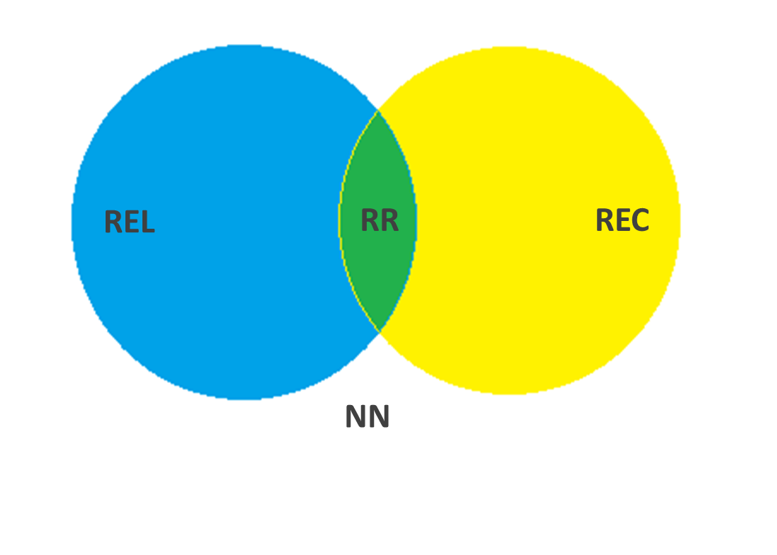
\includegraphics[width=0.5\textwidth]{./sri_03.png}
	\end{center}
	\caption{Clasificación de los documentos después de una consulta.}
	\label{fig:docSet}
\end{figure}

Donde:
\begin{itemize}
    \item {\bf REL:} Conjunto de documentos relevantes.
    \item {\bf REC:} Conjunto de documentos recuperados.
    \item {\bf RR:} Conjunto de documentos relevantes recuperados.
    \item {\bf NN:} Conjunto de documentos no relevantes no recuperados.
\end{itemize}

Sobre esta partición de conjuntos se aplican varias medidas de evaluación, con
las cuales se verifican la efectividad del modelo, las mismas son:

\begin{itemize}
    \item Precisión
    \item Recobrado (Recall)
    \item Medida F
    \item Medida F1
\end{itemize}

Estas medidas, aunque efectivas, no tienen en cuanta el \emph{ranking} de los
documentos, por lo que para una mayor efectividad del modelo se emplean otras
dos medidas para un mejor rendimiento, las cuales son:

\begin{itemize}
    \item R-Precisión
    \item Fallout 
\end{itemize}

Se incluyen en el modelo, además, opciones de comparación entre varias
colecciones, con el fin de realizar análisis entre las mismas.